\documentclass[10pt]{beamer}
\usetheme[
%%% option passed to the outer theme
%    progressstyle=fixedCircCnt,   % fixedCircCnt, movingCircCnt (moving is deault)
  ]{Feather}
  
% If you want to change the colors of the various elements in the theme, edit and uncomment the following lines

% Change the bar colors:
%\setbeamercolor{Feather}{fg=red!20,bg=red}

% Change the color of the structural elements:
%\setbeamercolor{structure}{fg=red}

% Change the frame title text color:
%\setbeamercolor{frametitle}{fg=blue}

% Change the normal text color background:
%\setbeamercolor{normal text}{fg=black,bg=gray!10}

%-------------------------------------------------------
% INCLUDE PACKAGES
%-------------------------------------------------------

\usepackage[utf8]{inputenc}
\usepackage[italian]{babel}
\usepackage{helvet}
\usepackage{listings}
\usepackage{xcolor}
\usepackage{graphicx}

%-------------------------------------------------------
% DEFFINING AND REDEFINING COMMANDS
%-------------------------------------------------------

% colored hyperlinks
\newcommand{\chref}[2]{
  \href{#1}{{\usebeamercolor[bg]{Feather}#2}}
}

%-------------------------------------------------------
% INFORMATION IN THE TITLE PAGE
%-------------------------------------------------------

\title[] % [] is optional - is placed on the bottom of the sidebar on every slide
{ % is placed on the title page
      \textbf{Progetto del corso Ingegneria di Internet e del Web a.a. 2017-2018}
}

\subtitle[Progetto del corso Ingegneria di Internet e del Web a.a. 2017-2018]
{
      \textbf{}
}

\author[Andrea Graziani - matricola 0189326]
{      Andrea Graziani - matricola 0189326 \\
      {}
}

\institute[]
{
      Facoltà di Ingegneria Informatica \\
      Università degli Studi di Roma Tor Vergata \\
  
  %there must be an empty line above this line - otherwise some unwanted space is added between the university and the country (I do not know why;( )
}

\date{\today}

% ----------------------------------------------------------------------------------------- %
% Usato per personalizzare l'ambiente 'listings'...
% ----------------------------------------------------------------------------------------- %
\lstset{
language=C,
basicstyle=\tiny\ttfamily,			
keywordstyle=\color{blue},
commentstyle=\color{gray},			
stringstyle=\color{black},			
numbers=left,						
numberstyle=\tiny,					
stepnumber=1,						
breaklines=true						
}

%-------------------------------------------------------
% THE BODY OF THE PRESENTATION
%-------------------------------------------------------

\begin{document}

%-------------------------------------------------------
% THE TITLEPAGE
%-------------------------------------------------------

{\1% % this is the name of the PDF file for the background
\begin{frame}[plain,noframenumbering] % the plain option removes the header from the title page, noframenumbering removes the numbering of this frame only
  \titlepage % call the title page information from above
\end{frame}}

% ----------------------------------------------------------------------------------------- %
\section{Architettura}
% ----------------------------------------------------------------------------------------- %

% ----------------------------------------------------------------------------------------- %
\subsection{Un'applicazione client-server con architettura a 2 livelli}
\begin{frame}{Architettura dell'applicazione}{Un'applicazione client-server con architettura a 2 livelli}
% ----------------------------------------------------------------------------------------- %

L'applicazione di rete sviluppata è di tipo \textbf{client-server con architettura a 2 livelli} in cui è prevista l'esistenza di: 

\begin{itemize}
\vspace*{10px}
\item Un \textbf{client} ossia l'entità che, incorporando tutta la logica applicativa che rende operativa l'applicazione (\textit{business logic}), accede ai servizi o alle risorse di un'altra componente, detta server. 
\vspace*{10px}
\item Un \textbf{server} ovvero l'entità incaricata di soddisfare le richieste di servizio provenienti dai client.
\end{itemize}



\end{frame}


% ----------------------------------------------------------------------------------------- %
\subsection{Un approccio concorrente}
\begin{frame}{Architettura dell'applicazione}{Un approccio concorrente}
% ----------------------------------------------------------------------------------------- %

\begin{block}{L'impraticabilità di un server iterativo}
Sebbene di semplice implementazione, un server di tipo \textbf{iterativo} non è adatto quando l'elaborazione delle richieste dei client richiede "\textit{molto tempo}" perché ciò comporta \textbf{tempi di attesa molto lunghi}.
\end{block}

\begin{block}{I vantaggi di un server concorrente}

In un server di tipo \textbf{concorrente} il compito di gestire e soddisfare le richieste ricevute dai client viene affidata ad un processo (o \textit{thread}) \textbf{distinto} da quello principale. Ciò consente di: 
\begin{itemize}
\item Gestire più richieste contemporaneamente.
\item Ridurre i tempi di attesa.
\item Permettere al processo server di poter continuare a ricevere ed elaborare nuove richieste.
\end{itemize}

\end{block}

\end{frame}

% ----------------------------------------------------------------------------------------- %
\subsection{Il processo server}
\begin{frame}{Architettura dell'applicazione}{Il processo server}
% ----------------------------------------------------------------------------------------- %

Se si analizza il codice della funzione \texttt{start\_server()} è facile intuire che il lavoro svolto dal \textbf{processo server} si articola in:

\begin{description}


\item[Inizializzazione della socket di ascolto] Necessaria per poter ricevere messaggi di richiesta dai client;
\item[Caricamento metadati] Questa fase prevede il caricamento di una serie di informazioni utili a soddisfare richieste di tipo \texttt{list};
\item[Fase di ascolto] Il processo server rimane in attesa dell'arrivo di un messaggio di richiesta sulla socket di ascolto precedentemente creata.
\item[Creazione del thread] Alla ricezione di un messaggio di richiesta viene creato un nuovo thread a cui affidare il compito di gestire e soddisfare la richiesta ricevuta. Successivamente il processo server ritorna in fase di ascolto.
\end{description}

\end{frame}

% ----------------------------------------------------------------------------------------- %
\subsection{Il processo server 2}
\begin{frame}{Architettura dell'applicazione}{Il processo server - Inizializzazione della socket di ascolto}
% ----------------------------------------------------------------------------------------- %

Da un punto di vista implementativo la \textbf{fase di inizializzazione della socket di ascolto} avviene attraverso l'esecuzione della funzione \texttt{\_\_server\_initialization} che prevede:

\begin{enumerate}
\item L'esecuzione della chiamata di sistema \\ \texttt{socket(int domain, int type, int protocol)} dove:
\begin{enumerate}
\vspace*{10px}
\item Il parametro \texttt{domain} indica il \textbf{dominio di comunicazione} cioè specifica la famiglia dei protocolli che verranno usati nella comunicazione. \\ Il dominio scelto è \texttt{AF\_INET} che designa il \textbf{protocollo IPv4}.
\vspace*{10px}
\item Il parametro \texttt{type} specifica il \textit{tipo di socket} ed è utilizzato per specificare \textbf{la semantica della comunicazione}. \\ Il tipo scelto è stato \texttt{SOCK\_DGRAM} che una forma di comunicazione \textbf{basata su datagrammi}, \textbf{senza connessione}, \textbf{inaffidabile} e che può inviare \textbf{messaggi di lunghezza prefissata}.
\vspace*{10px}
\item Il parametro \textbf{protocol} specifica il particolare protocollo da utilizzare con la socket specificata. \\
\end{enumerate}

\end{enumerate}

\end{frame}

% ----------------------------------------------------------------------------------------- %
\subsection{Il processo server 3}
\begin{frame}[fragile]{Architettura dell'applicazione}{Il processo server - Inizializzazione della socket di ascolto}
% ----------------------------------------------------------------------------------------- %

Una volta creata una socket mediante la chiamata di sistema \texttt{socket} occorre assegnarle un indirizzo mediante la chiamata di sistema \texttt{bind} che permette di assegnare alla socket l'indirizzo specificato da una struttura dati di tipo \texttt{sockaddr}.

\begin{lstlisting}
// Set address family that is used to designate the type of addresses that socket 
// can communicate with: in this case, Internet Protocol v4 addresses */
servaddr.sin_family = AF_INET;
/* Server accepts request on any network interface */
servaddr.sin_addr.s_addr = htonl(INADDR_ANY);

/* Specify port 'SERVER_PORT' converting them from host byte order to network byte order. */
if (main_process) {
	servaddr.sin_port = htons(SERVER_COMMAND_PORT);

	// allow reuse of local address if there is not an active listening
	// socket bound to the address
	int reuse = 1;
	if (setsockopt(sockfd, SOL_SOCKET, SO_REUSEADDR, &reuse, sizeof(int)) == -1)
		exit_failure("setsockopt");

} else
	servaddr.sin_port = 0;

/* Bind the socket to server address */
if (bind(sockfd, (struct sockaddr*) &servaddr, sizeof(servaddr)) == -1)
	exit_failure("bind");
\end{lstlisting}

\end{frame}


% ----------------------------------------------------------------------------------------- %
\subsection{Il processo client}
\begin{frame}[fragile]{Architettura dell'applicazione}{Il processo client}
% ----------------------------------------------------------------------------------------- %

\begin{block}{Messaggi di richiesta}
Un client può inoltrare richieste di servizio al server attraverso l'invio di un apposito \textbf{messaggio di richiesta} sfruttando la socket di ascolto. 
\end{block}

\vspace*{10px}
Un messaggio di richiesta è modellato dalla struttura dati di tipo \texttt{RequestPacket} la quale specifica il tipo, i parametri e le modalità di esecuzione di una data richiesta.

\begin{lstlisting}[frame=lines, caption={Implementazione della struttura \texttt{RequestPacket}}]
typedef struct request_client_packet {

	Settings client_setting;
	char request_type;
	char request_type_argument[NAME_MAX];

} RequestPacket;
\end{lstlisting}


\end{frame}

% ----------------------------------------------------------------------------------------- %
\subsection{Il processo client 2}
\begin{frame}[fragile]{Architettura dell'applicazione}{Il processo client}
% ----------------------------------------------------------------------------------------- %

Analizzando la funzione \texttt{client\_start} è facile intuire che l'invio di un messaggio di richiesta e dunque l'inizio di una trasmissione prevede:

\begin{itemize}
\item L'inizializzazione di una struttura dati denominata \texttt{RequestPacket}.
\item L'invio della suddetta struttura al server attraverso l'ausilio di una struttura di tipo \texttt{DataNetwork}.
\item Attesa della risposta dal server; in caso di mancata risposta occorre rinviare un nuovo messaggio di richiesta.
\end{itemize}



\end{frame}



% ----------------------------------------------------------------------------------------- %
\subsection{Il processo client 3}
\begin{frame}[fragile]{Architettura dell'applicazione}{Il processo client}
% ----------------------------------------------------------------------------------------- %

\begin{block}{La struttura dati \texttt{DataNetwork}}
Una struttura dati di tipo \texttt{DataNetwork} rappresenta tecnicamente un contenitore per tutte le informazioni necessarie per comunicare con un host tra cui l'\textbf{indirizzo IP} e il \textbf{numero di porta}. 
\end{block}

\begin{lstlisting}[frame=lines, caption={Implementazione della struttura \texttt{DataNetwork}}]
typedef struct data_network {

	/* Socket file descriptor */
	int socket_fd;
	/* Internet socket address */
	struct sockaddr_in address;
	/* Internet socket address length */
	socklen_t address_len;

} DataNetwork;

\end{lstlisting}
\end{frame}

% ----------------------------------------------------------------------------------------- %
\subsection{Il processo client 4}
\begin{frame}[fragile]{Architettura dell'applicazione}{Il processo client}
% ----------------------------------------------------------------------------------------- %

\begin{block}{Problema}
Il server UDP deve poter scambiare più di un pacchetto con il client per poter soddisfarne le richieste. Il problema è che \textbf{l'unico numero di porta noto} al client per poter comunicare con il server è, sfortunatamente, \textbf{la stessa porta utilizzata da quest'ultimo per ricevere nuove richieste}.
\end{block}

\end{frame}

% ----------------------------------------------------------------------------------------- %
\subsection{Il processo client 5}
\begin{frame}[fragile]{Architettura dell'applicazione}{Il processo client}
% ----------------------------------------------------------------------------------------- %

\begin{block}{Soluzione}
I thread incaricati di soddisfare le richieste hanno il compito di \textbf{creare un'apposita socket di supporto} eseguendo il \textbf{binding su una porta effimera} e utilizzando quel socket per inviare e ricevere i successivi messaggi con un client.
\end{block}

\vspace*{10px}
Il client deve guardare \textbf{il numero di porta della prima risposta del server} e dunque inviare i pacchetti successivi a quella porta. \\

\vspace*{10px}
Da un punto di vista implementativo ciò è reso possibile dalla funzione \texttt{\_\_receive\_datagram} la quale provvede ad \textbf{aggiornare il contenuto della struttura \texttt{DataNetwork}} dopo la ricezione della prima risposta. Tutto ciò permette al client di \textbf{ignorare tutti quei pacchetti non provenienti dal processo server con cui interagisce}.
\end{frame}



% ----------------------------------------------------------------------------------------- %
\subsection{Schema di funzionamento}
\begin{frame}{Architettura dell'applicazione}{Schema di funzionamento}
% ----------------------------------------------------------------------------------------- %

\begin{figure}
\centering
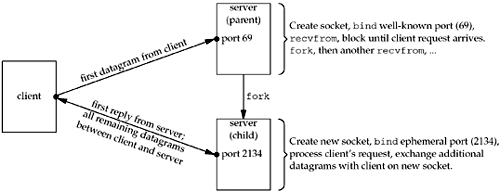
\includegraphics[width=\textwidth]{Concorrente}
\caption{Schema del funzionamento di un server concorrente.}
\label{fig:Concorrente}
\end{figure}

\end{frame}



% ----------------------------------------------------------------------------------------- %
\section{Servizio di trasmissione affidabile}
% ----------------------------------------------------------------------------------------- %

% ----------------------------------------------------------------------------------------- %
\subsection{Introduzione}
\begin{frame}[fragile]{Servizio di trasmissione affidabile}{}
% ----------------------------------------------------------------------------------------- %

\begin{block}{Obiettivo}
Per i scopi della nostra applicazione abbiamo bisogno di realizzare un \textbf{protocollo applicativo} che fornisca un \textbf{servizio di trasmissione dati affidabile} basandosi, tuttavia, su un protocollo di trasporto che offra, invece, un servizio di comunicazione inaffidabile (detto anche \textit{best effort}).
\end{block}

\vspace*{10px}

Garantire un servizio di trasmissione dati affidabile richiede di:

\begin{itemize}
\item Gestire in modo adeguato la presenza di errori sui bit dei pacchetti trasmessi.
\item Riuscire a rilevare e poi a gestire lo smarrimento di uno o più pacchetti.
\end{itemize}

\end{frame}

% ----------------------------------------------------------------------------------------- %
\subsection{La necessità dei feedback}
\begin{frame}{Servizio di trasmissione affidabile}{}
% ----------------------------------------------------------------------------------------- %

Come in moltissimi protocolli di comunicazione, il mittente e il destinatario devono essere in grado di potersi scambiare appositi \textbf{messaggi di notifica} per gestire situazioni di errore o smarrimento dei dati trasmessi. \\

\vspace*{10px}
Infatti questi messaggi di notifica risultano fondamentali per due importanti motivi:
\begin{itemize}
\item Garantire il corretto funzionamento del protocollo applicativo il quale, in accordo alle specifiche progettuali, deve simulare un protocollo di trasmissione a \textbf{ripetizione selettiva}. Infatti \textbf{l 'unico modo che ha il mittente per sapere se un pacchetto sia stato ricevuto correttamente o meno consiste nel \textit{feedback} esplicito del destinatario.} 
\item Individuare un pacchetto smarrito in basa alla mancata o eccessivamente ritardata ricezione del messaggio di notifica proveniente dal destinatario.
\end{itemize}

\end{frame}

% ----------------------------------------------------------------------------------------- %
\subsection{I messaggi di controllo}
\begin{frame}[fragile]{Servizio di trasmissione affidabile}{I messaggi di controllo}
% ----------------------------------------------------------------------------------------- %

\begin{block}{I messaggi di controllo}
Nella terminologia usata dal nostro protocollo i messaggi di notifica scambiati dagli host sono rappresentati dai cosiddetti \textbf{messaggi di controllo}. 
\end{block}

Da un punto di vista implementativo i messaggi di controllo, modellati dalla struttura \textbf{\texttt{ControlDatagram}}, vengono utilizzati per:

\begin{enumerate}
\item Inviare al mittente un riscontro (o ACK, anche detto \textit{acknowledgement}) per i pacchetti ricevuti in modo corretto compatibilmente con il protocollo di trasmissione SR.
\item Gestire le procedure di instaurazione e chiusura delle trasmissioni.
\end{enumerate}

\begin{lstlisting}[frame=lines, caption={Implementazione della struttura \texttt{ControlDatagram}}]
typedef struct control_datagram {
	char type;
	char n;
} ControlDatagram;
\end{lstlisting}


\end{frame}


% ----------------------------------------------------------------------------------------- %
\subsection{Gestione delle ritrasmissioni}
\begin{frame}[fragile]{Servizio di trasmissione affidabile}{Rilevare lo smarrimento dei pacchetti}
% ----------------------------------------------------------------------------------------- %

\begin{block}{Come rilevare un pacchetto smarrito?}
Come abbiamo detto in precedenza se dopo la trasmissione di un certo pacchetto il mittente non ricevesse alcun riscontro da parte del destinatario dopo un certo \textit{lasso di tempo}, il mittente considera il suddetto pacchetto come \textit{smarrito} e procede alla \textit{ritrasmissione} di quest'ultimo. 
\end{block}

\vspace*{10px}

\begin{block}{Quanto deve essere lungo questo \textit{lasso di tempo}?}
Ovviamente l'intervallo di timeout dovrebbe essere più grande del tempo di andata e ritorno del segnale sulla connessione per evitare timeout prematuri o troppo ritardati. \\ L'algoritmo usato per il calcolo della lunghezza dell'intervallo di timeout è analogo a quello usato nel protocollo di trasporto TPC.
\end{block}

\end{frame}

% ----------------------------------------------------------------------------------------- %
\subsection{Gestione delle ritrasmissioni 2}
\begin{frame}[fragile]{Servizio di trasmissione affidabile}{Le ritrasmissioni}
% ----------------------------------------------------------------------------------------- %

Dovendo simulare un protocollo di comunicazione SR, dobbiamo associare ad ogni pacchetto da trasmettere un timer dedicato capace di segnalare al mittente l'avvenuta scadenza di un dato lasso di tempo. \\
\vspace*{10px}
Inoltre il mittente deve essere in grado di:

\begin{itemize}
\item Inizializzare un timer ogni volta che invia un pacchetto.
\item Rispondere adeguatamente all'interrupt generato dal timer in caso di timeout procedendo quindi alla ritrasmissione del pacchetto smarrito e reinizializzare il timer.
\item Disabilitare il timer quando il mittente riceve un riscontro positivo da parte del destinatario.
\end{itemize} 

\end{frame}


% ----------------------------------------------------------------------------------------- %
\subsection{Gestione delle ritrasmissioni 3}
\begin{frame}[fragile]{Servizio di trasmissione affidabile}{La struttura \texttt{DatagramTimer}}
% ----------------------------------------------------------------------------------------- %

L'associazione tra uno specifico pacchetto con un timer avviene mediante l'ausilio di un'apposita struttura dati denominata \texttt{DatagramTimer}.

\begin{lstlisting}[frame=lines, caption={Implementazione della struttura \texttt{DatagramTimer}}]
typedef struct datagram_timer {
	void *Datagram_ptr;
	DataNetwork *DataNetwork_ptr;
	
	char *abort_trasmission_ptr;
	char datagram_type;
	
	timer_t timer;
	char times_retrasmitted;
	struct itimerspec timervals;
	struct timespec sending_time;
	struct timespec receiving_time;
} DatagramTimer;
\end{lstlisting}


\end{frame}

% ----------------------------------------------------------------------------------------- %
\subsection{Gestione delle ritrasmissioni 4}
\begin{frame}[fragile]{Servizio di trasmissione affidabile}{Inizializzazione della struttura \texttt{DatagramTimer}}
% ----------------------------------------------------------------------------------------- %

L'associazione di uno pacchetto con un timer consiste nell'eseguire una procedura di inizializzazione di un oggetto \texttt{DatagramTimer} che prevede le seguenti fasi:

\begin{itemize}
\item Associazione del pacchetto;
\item Configurazione handler ossia dichiarazione della procedura da seguire in caso di timeout;
\item Configurazione della struttura \texttt{sigevent} durante la quale viene specificata le modalità attraverso cui l'applicazione debba essere avvisata dell'avvenuto timeout;
\item Creazione del timer logico in accordo alle API POSIX;
\end{itemize}

\end{frame}


% ----------------------------------------------------------------------------------------- %
\subsection{Gestione delle ritrasmissioni 5}
\begin{frame}[fragile]{Servizio di trasmissione affidabile}{Inizializzazione della struttura \texttt{DatagramTimer}}
% ----------------------------------------------------------------------------------------- %

\begin{lstlisting}
void DatagramTimer_init(DatagramTimer *DatagramTimer_obj, void **Datagram_ptr, DataNetwork **DataNetwork_ptr, char *abort_trasmission_ptr,
		char datagram_type, void (*handler)(int, siginfo_t*, void*)) {

	struct sigevent sev;
	struct sigaction sa;

	/* Configuration 'DatagramTimer' */
	if (DataNetwork_ptr != NULL)
		DatagramTimer_obj->DataNetwork_ptr = *DataNetwork_ptr;
	if (Datagram_ptr != NULL)
		DatagramTimer_obj->Datagram_ptr = *Datagram_ptr;

	DatagramTimer_obj->abort_trasmission_ptr = abort_trasmission_ptr;
	DatagramTimer_obj->datagram_type = datagram_type;

	/* Establish handler for notification signal */
	sa.sa_flags = SA_SIGINFO;
	sa.sa_sigaction = handler;
	sigemptyset(&sa.sa_mask);
	sigaddset(&sa.sa_mask, SIGRTMAX);
	if (sigaction(SIGRTMAX, &sa, NULL) == -1)
		exit_failure("sigaction");

	/* Configuration structure to transport application-defined values with signals. */
	sev.sigev_notify = SIGEV_THREAD_ID;
	sev._sigev_un._tid = syscall(SYS_gettid);
	sev.sigev_signo = SIGRTMAX;
	sev.sigev_value.sival_ptr = DatagramTimer_obj;

	/* Create new per-process timer using CLOCK_ID. */
	if (timer_create(CLOCK_REALTIME, &sev, &DatagramTimer_obj->timer) == -1)
		exit_failure("timer_create");
}
\end{lstlisting}

\end{frame}


% ----------------------------------------------------------------------------------------- %
\section{Gestione della trasmissione dati}
% ----------------------------------------------------------------------------------------- %


% ----------------------------------------------------------------------------------------- %
\subsection{Schema generale}
\begin{frame}[fragile]{Gestione della trasmissione dati}{Schema generale}
% ----------------------------------------------------------------------------------------- %


\begin{block}{Fasi della trasmissione dati}
Per la trasmissione dei dati fra host il protocollo applicativo prevede l'esecuzione delle seguenti operazioni:

\begin{itemize}
\item Inizializzazione della trasmissione;
\item Instaurazione della trasmissione;
\item Trasmissione dati;
\item Chiusura della trasmissione;
\end{itemize}

\end{block}
\end{frame}

% ----------------------------------------------------------------------------------------- %
\subsection{Inizializzazione della trasmissione}
\begin{frame}[fragile]{Gestione della trasmissione dati}{Inizializzazione della trasmissione}
% ----------------------------------------------------------------------------------------- %

Durante questa fase devono essere allocate e inizializzate tutte le strutture dati necessarie per eseguire la trasmissione tra cui:

\begin{itemize}
\item Un \textit{buffer di ricezione} (lato client) e un \textit{buffer di invio} (lato server) entrambi di dimensione $N$. Ricordiamo che la relazione ottimale tra la dimensione del buffer $N$ e la dimensione dell'apertura della finestra di spedizione
$W$ è:
\[
N = 2W
\]

\item Un buffer di dimensione $N$ usato per ospitare oggetti di tipo \texttt{DatagramTimer} necessari per l'associazione tra timer e pacchetti.
\item Un oggetto di tipo \texttt{TimeInfo}.
\item Un oggetto di tipo \texttt{NetworkStatistics}.
\end{itemize}

\end{frame}

% ----------------------------------------------------------------------------------------- %
\subsection{Instaurazione della trasmissione}
\begin{frame}[fragile]{Gestione della trasmissione dati}{Instaurazione della trasmissione}
% ----------------------------------------------------------------------------------------- %


Questa fase è necessaria per segnalare l'inizio di una trasmissione ed è utile per distinguere correttamente più trasmissioni consecutive eseguite tra una stessa coppia di host. \\
\vspace*{10px}

Questa fase, similmente a quanto avviene nella fase di connessione in TCP, prevede la trasmissione di tre opportuni messaggi di controllo: si può parlare dunque di \textbf{handshake a tre vie} (\textit{three-way handshake}).


\end{frame}

% ----------------------------------------------------------------------------------------- %
\subsection{Trasmissione dati}
\begin{frame}[fragile]{Gestione della trasmissione dati}{Trasmissione dati}
% ----------------------------------------------------------------------------------------- %


Il protocollo suddivide la trasmissione dei dati nelle seguenti operazioni:

\begin{itemize}
\item Lettura dal \textit{file system} e incapsulamento dati;
\item Invio pacchetto dati previa attivazione timer ad esso associato rispettando le regole del protocollo SR;
\item Gestione dei riscontri ricevuti previa disattivazione dei timer associati a pacchetti inviati con successo e aggiornamento delle variabili della trasmissione compatibilmente con il protocollo SR;
\item Eventuale ritrasmissione di pacchetti smarriti;
\end{itemize}


\end{frame}

% ----------------------------------------------------------------------------------------- %
\subsection{Chiusura della trasmissione}
\begin{frame}{Gestione della trasmissione dati}{Chiusura della trasmissione}
% ----------------------------------------------------------------------------------------- %


La chiusura della trasmissione avviene solo quando sono entrambe verificate le seguenti condizioni: 

\begin{itemize}
\item Il mittente non ha più dati da inviare al destinatario;
\item Il mittente rileva che anche l'ultimo pacchetto inviato ha ricevuto un riscontro positivo;
\end{itemize}

\vspace*{10px}
Il protocollo prevede l'invio di appositi messaggi di controllo (\texttt{FIN}, \texttt{FIN\_ACK}, \texttt{CLS}) per terminare correttamente la trasmissione.


\end{frame}

{\1
\begin{frame}[plain,noframenumbering]
  \finalpage{Grazie per l'attenzione!}
\end{frame}}


\end{document}